\documentclass[a4paper]{article}

\usepackage[utf8]{inputenc}
\usepackage[T1]{fontenc}
\usepackage{textcomp}
\usepackage[english]{babel}
\usepackage{amsmath, amssymb}
\usepackage{physics}


% figure support
\usepackage{import}
\usepackage{xifthen}
\pdfminorversion=7
\usepackage{pdfpages}
\usepackage{transparent}
\newcommand{\incfig}[1]{%
	\def\svgwidth{\columnwidth}
	\import{./figures/}{#1.pdf_tex}
}

\pdfsuppresswarningpagegroup=1
\title{PH 550 - Soft Matter Physics}
\begin{document}
\section{Introduction}
AKA Soft Condensed Matter Physics (MC mai ghoom phir ke CMP pe aa gya).  Course content
\begin{enumerate}
	\item Intro to soft matter
	\item Viscoelasticity
	\item Colloids
	\item Polymers
	\item Surfactants
	\item Liquid Crystals
\end{enumerate}

Books
\begin{itemize}
	\item Soft Matter Physics (Richard Jones)
	\item Soft Matter Physics (Masao Doi)
	\item Introduction to the Theory of Soft Matter (Jonathan Selinger) [liquid crystals]
\end{itemize}

So, there's three adjectives in front of the word `Physics'.

\subsection{Matter}
Composed of atoms or molecules. Matter refers to collections of atoms
and molecules. Don't go about referring to a single atom as `matter'.

It is expected that when we say `matter', we have a very large ($\approx N_A$) number
of building components. 

So, how does  one go about dealing with such
systems? Statistical physics. Your Hamiltonian formalism and Newton's
equations will shit the bed.

Solid systems and gaseous systems are easy to deal with for Physicists,
because some really neat approximations can be made. In liquids, however
potential energy $\approx$ kinetic energy.

[Missed some part of the lecture]

An example of Helium's phase diagram was given. There is a critical
pressure below which it cannot exist in the liquid state. Point was
$P>0$ for the existence of liquid, or something like that. You need
pressure for  the existence of liquids.

You see, the world is not just made up of solid, liquid and gas only.
Like what the fuck even is the phase of toothpaste and shampoo??

\begin{figure}[h]
	\centering
	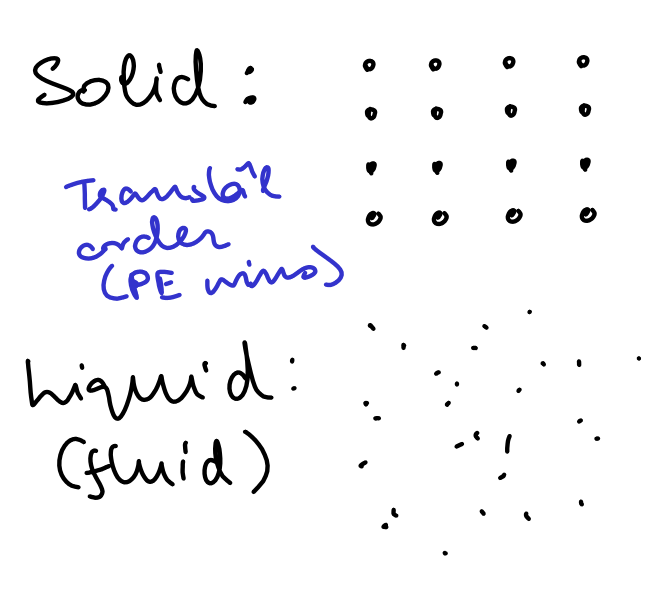
\includegraphics[width=0.8\textwidth]{figures/order.png}
	\caption{Fluids vs solids - order}
	\label{fig:figures-order-png}
\end{figure}

\begin{itemize}
	\item Solid
		\begin{itemize}
			\item Translational order
			\item translationally broken symmetry
			\item  broken rotational symmetry
		\end{itemize}
	\item Fluid
		\begin{itemize}
			\item Translationally disordered
			\item translationally symmetric
			\item rotational symmetries  preserved
		\end{itemize}
\end{itemize}

Deformations are not energetically favourable in solids and hence
any attempts to move  particles by shearing, compressing etc will
result in strong restoring forces.

Fluids on the other hand have 0 elastic moduli

Then  we have soft matter  systems, where the elastic moduli are
somewhere in between the above two  cases.

Systems like liquid crystals  are again quite unique because 
\begin{itemize}
	\item  Rotational order
	\item No translational order
\end{itemize}

BTW time scales matter. Phase diagrams don't  show time, only
thermodynamic parameters. But, we generally think of different phases
like solids, liquids etc in terms of their response funcions - their dynamics.
If something is hard, it's solid. If something flows, it's liquid.
Phase diagrams do not really capture the dynamics  properly.

\subsection{Grading}
\begin{itemize}
	\item Home assignments - 33\%
	\item Midsem - 33\%
	\item Endsem - 33\%
\end{itemize}
\end{document}
